\documentclass[12pt]{article}
\usepackage{amsmath}
\usepackage{amsfonts}
\usepackage{graphicx}
\DeclareGraphicsExtensions{.pdf,.png,.jpg}
\usepackage{algpseudocode}

\newtheorem{theorem}{Theorem}[section]
\newtheorem{lemma}[theorem]{Lemma}
\newtheorem{definition}[theorem]{Definition}


\title{Uncovered Pixels in 2D}
\date{}
\begin{document}
  \maketitle

  By setting the number of random points in the whole space from 200 ~ 7000, repeating 5 times, our algorithm collected some data about uncovered pixels in 2D space. The 2D space is 800x800 large, and all discs sampled by our algorithm have radius at least 10. The numbers in the charts below are the average number of 5 experiments.
  
  In the charts you are going to see, the x-axis indicates the number of random points in the whole space, the y-axis indicates the distance from such a point to obstacles or the boundary of the world, while the z-axis is the amount of pixels. For example, (7000, 10, 8) means, with initially 7000 points, our algorithm left 8 pixels that are 10 distance away from obstacles or boundaries.
  
  \section{Plotting Overview}
  
  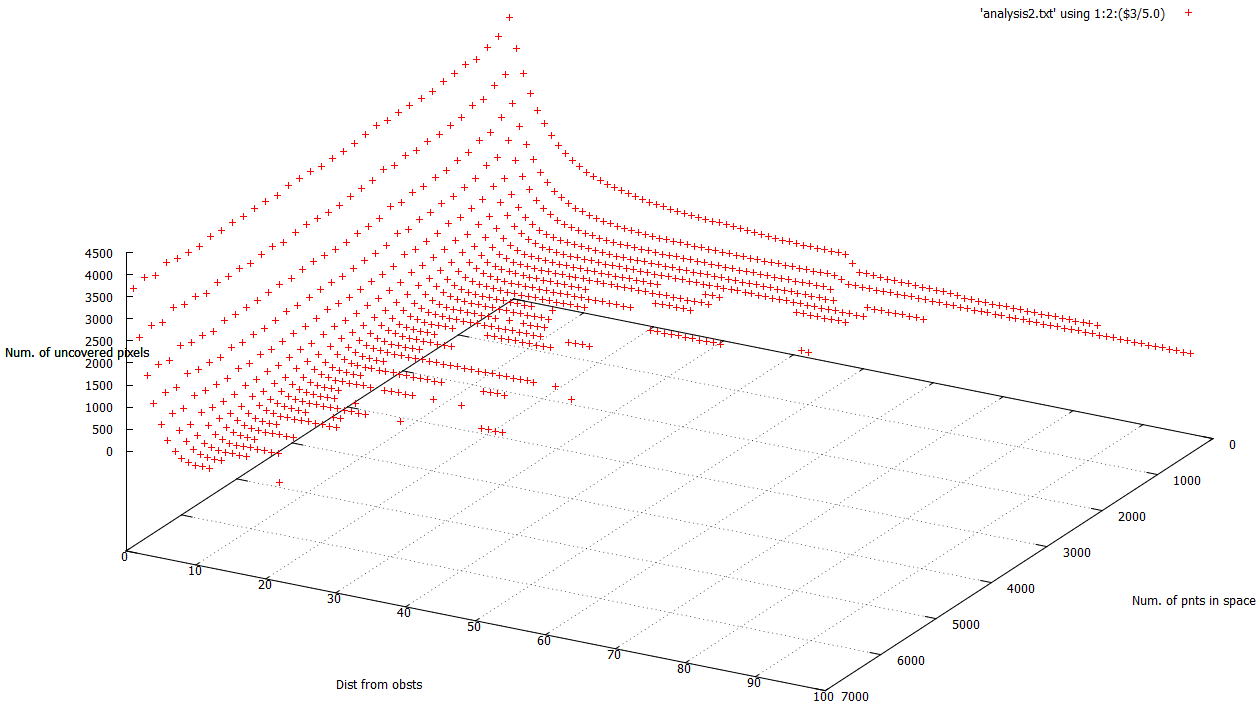
\includegraphics[scale=0.5]{overview.PNG}
  
  As we can see in the picture, with more initial random points, we are expecting less far-from-obstacle points to be uncovered by discs. But still, we observe a few points exception points, which means our algorithm will left some holes in the free space to be uncovered, although such holes are really small. Increasing the number of random points seems to have the ability of reducing such exception points. There is no uncovered point that is 10 distance away from obstacles with 7000 initial random points.
  
  \section{Grown Obstacles}
  By setting the minimum radius of discs to be 10, we are expecting 0 point that is 10 distance away from obstacles to be uncovered. Our experiment seems to be supporting the theory. The graph below shows the number of points that have 10 to 30 clearance with different initial random points.
  
  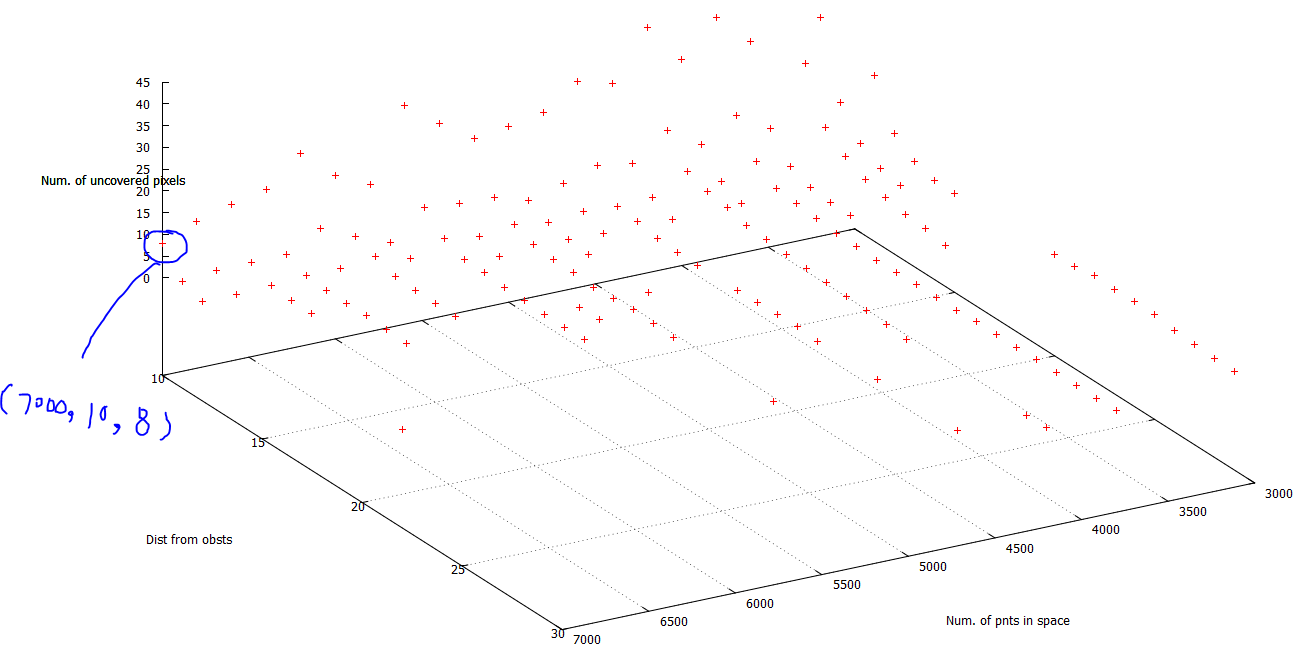
\includegraphics[scale=0.45]{7000_10_8.PNG}
  
  With 7000 random points, there are still 8 points that are 10 distance away from obstacles, although we are expecting the number to be 0. This is probably not unacceptable, because the algorithm does not guarantee to sample every point on the boundary of existing discs. And 8 points out of 800x800 points is not too bad.
  
  \section{The Trend}
  
  By projecting data to x-y plane, we can see the trend of reducing far-from-obstacle points.
  
  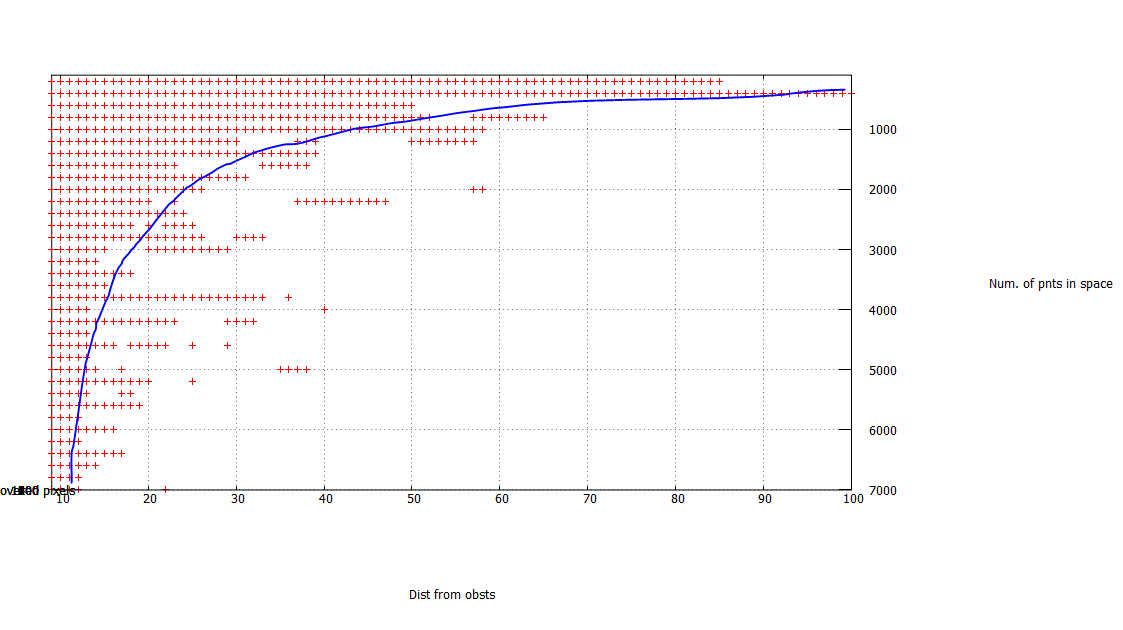
\includegraphics[scale=0.6]{overhead_view.PNG}
  
    
\end{document}
  